\chapter{Results and Discussion}

\section{Overview}

This chapter reports the experimental results produced by the pipeline described in Chapter 4. The aim is to answer the research questions defined in Chapter 3 by examining whether structured prompts reduce over-correction risk while maintaining grammatical correction performance.

The chapter is organised around six analyses. Experiment 1 refines prompt variants within each prompt family. Experiment 2 compares the selected baseline, instruction-constrained, role-based, and few-shot prompts. Experiment 3 examines sentence-length effects. Experiment 4 tests the robustness of OCI under alternative weighting schemes. Experiment 5 analyses the trade-off between ERRANT $F_{0.5}$ and OCI. Experiment 6 uses selected examples to inspect how potential over-correction appears at sentence level.

Throughout this chapter, ERRANT $F_{0.5}$ is used to represent grammatical correction quality, while OCI is used as the main indicator of over-correction risk. As explained in Chapter 4, OCI is a comparative indicator rather than a direct judgement that every edit is unnecessary. The results are therefore interpreted using OCI together with ERRANT scores, edit distance, and qualitative examples.

\section{Experiment 1: Prompt Refinement}

\subsection{Purpose}

Experiment 1 was used to identify the strongest prompt variant within each prompt family before the main comparison. This step was necessary because small wording changes can affect how much an LLM edits learner writing. Two prompts may appear similar but still produce different balances between grammatical correction and preservation of the original sentence.

\subsection{Procedure}

This experiment used 500 learner sentences from the prepared W\&I + LOCNESS subset. Each sentence was processed using the baseline prompt and several variants from the instruction-constrained, role-based, and few-shot prompt families. For every output, ERRANT precision, recall, $F_{0.5}$, and OCI were calculated.

The aim of this stage was prompt selection rather than final evaluation. The strongest candidate from each structured prompt family was carried forward into Experiment 2, while the baseline prompt was retained as the control condition.

\subsection{Results}

\begin{table}[htbp]
    \centering
    \caption{Prompt refinement results for Experiment 1 -- all variants}
    \label{tab:exp1_prompt_refinement}
    \renewcommand{\arraystretch}{1.15}
    \begin{adjustbox}{max width=\textwidth}
    \begin{tabular}{lrrrr}
        \toprule
        \textbf{Condition} & \textbf{Precision} & \textbf{Recall} & \textbf{$F_{0.5}$} & \textbf{OCI (\%)} \\
        \midrule
        Baseline       & 42.71 & 52.32 & 44.34 & 1.40 \\
        \addlinespace
        Instruction v1 & 42.15 & 52.63 & 43.90 & 1.50 \\
        Instruction v2 & 53.54 & 39.01 & 49.83 & 0.98 \\
        Instruction v3 & 50.60 & 43.24 & 48.94 & 1.06 \\
        Instruction v4 & 52.82 & 39.63 & 49.52 & 1.05 \\
        \addlinespace
        Role v1        & 42.18 & 52.32 & 43.88 & 1.37 \\
        Role v2        & 44.77 & 50.77 & 45.85 & 1.36 \\
        Role v3        & 54.15 & 36.33 & 49.31 & 1.06 \\
        Role v4        & 55.03 & 38.39 & 50.64 & 1.05 \\
        \addlinespace
        Few-shot v1    & 44.37 & 51.29 & 45.60 & 1.51 \\
        Few-shot v2    & 45.27 & 51.39 & 46.38 & 1.49 \\
        Few-shot v3    & 45.49 & 52.01 & 46.66 & 1.54 \\
        Few-shot v4    & 54.47 & 43.34 & 51.81 & 1.12 \\
        \bottomrule
    \end{tabular}
    \end{adjustbox}
\end{table}

The baseline prompt achieved an $F_{0.5}$ score of 44.34 and an OCI of 1.40\%. Among the instruction-constrained prompts, Instruction v2 achieved the lowest OCI, 0.98\%, and an $F_{0.5}$ score of 49.83. Instruction v4 produced a similar $F_{0.5}$ score, 49.52, with OCI of 1.05\%. Role v4 achieved $F_{0.5}$ of 50.64 and OCI of 1.05\%. Few-shot v4 achieved the highest $F_{0.5}$ score in this experiment, 51.81, with OCI of 1.12\%.

\subsection{Discussion}

The refinement results show that prompt wording has a measurable effect on correction behaviour. The baseline result acts as a useful reference point because it shows that a simple request to correct grammar does not produce the strongest balance between accuracy and controlled editing.

Within the instruction-constrained family, Instruction v2 produced the strongest balance between correction accuracy and over-correction risk. It achieved the highest $F_{0.5}$ among the instruction variants, 49.83, and also the lowest OCI, 0.98\%. Instruction v4 was close in accuracy, with $F_{0.5}$ of 49.52, but its OCI was higher at 1.05\%. Although Instruction v4 stated the minimal-edit constraint more explicitly, including references to tone, style, vocabulary, and unnecessary word addition or removal, this did not translate into a lower over-correction risk score. This suggests that a more detailed constraint does not automatically produce more controlled correction behaviour. For this reason, Instruction v2 was selected as the instruction-constrained prompt to carry forward. This selection is based on the same evaluation logic used throughout the dissertation: prompt candidates are compared using both ERRANT $F_{0.5}$ and OCI, rather than by wording preference alone.

The role-based prompts show a slightly different pattern. Role v3 had marginally lower OCI than Role v4, but Role v4 achieved stronger grammatical correction performance, with $F_{0.5}$ of 50.64 compared with 49.31 for Role v3. Since the difference in OCI was small, Role v4 was selected as the role-based prompt because it provided the better balance between correction accuracy and over-correction risk. This choice also reflects the overall aim of the study: reducing over-correction is important, but not at the expense of substantially weaker grammatical correction performance.

The few-shot variants showed the clearest accuracy advantage. Few-shot v4 achieved the highest $F_{0.5}$ score in the refinement stage, 51.81, suggesting that examples helped the model follow the expected correction format. Its OCI, 1.12\%, was slightly higher than the best instruction-constrained and role-based variants, indicating a broader correction scope. However, it remained lower than the baseline OCI and provided the strongest grammatical correction performance overall. For this reason, Few-shot v4 was selected as the few-shot prompt for the main comparison.

These results justify the final candidate set used in the main strategy comparison: Instruction v2, Role v4, Few-shot v4, and the baseline. Since Experiment 1 is a refinement stage, it does not by itself prove that one prompt family is generally superior. Instead, it identifies the strongest representative from each structured prompt family so that they can be evaluated more directly in the following experiments.

\section{Experiment 2: Comparison of Prompting Strategies}

\subsection{Purpose}

Experiment 2 compares the final prompting strategies selected in Experiment 1. The purpose is to evaluate how different prompt designs influence the balance between grammatical correction performance and over-correction risk.

The aim is not only to identify which prompt achieves the highest correction score, but also to examine how each strategy affects editing behaviour. In particular, the experiment considers whether improvements in ERRANT $F_{0.5}$ are associated with higher or lower OCI, supported by edit-distance results.

\subsection{Procedure}

The same 500 learner sentences were processed under four prompt conditions: baseline, instruction-constrained, role-based, and few-shot. The instruction-constrained, role-based, and few-shot prompts correspond to the refined variants selected in Experiment 1.

Outputs were evaluated using the two evaluation paths implemented in Chapter 4. ERRANT precision, recall, and $F_{0.5}$ measured agreement with reference corrections. OCI was used as the over-correction risk indicator, while edit distance was reported as a direct surface-change measure. Since each sentence was evaluated under all prompt conditions, paired comparisons were also used to assess whether OCI differences were consistent across inputs.

\subsection{Results}

\begin{table}[htbp]
    \centering
    \caption{Comparison of final prompt strategies for Experiment 2}
    \label{tab:exp2_strategy_comparison}
    \renewcommand{\arraystretch}{1.15}
    \begin{adjustbox}{max width=\textwidth}
    \begin{tabular}{lrrrrrrl}
        \toprule
        \textbf{Condition} 
        & \textbf{Precision} 
        & \textbf{Recall} 
        & \textbf{$F_{0.5}$} 
        & \textbf{Mean OCI} 
        & \textbf{OCI (\%)} 
        & \textbf{Edit Dist.} 
        & \textbf{Interpretation} \\
        \midrule
        Baseline    
        & 40.98 & 52.73 & 42.89 & 0.01693 & 1.69 & 6.70 
        & Weak/inefficient \\

        Instruction 
        & 53.54 & 39.01 & 49.83 & 0.00989 & 0.99 & 5.53 
        & Conservative \\

        Role        
        & 55.03 & 38.39 & 50.64 & 0.01059 & 1.06 & 5.52 
        & Balanced \\

        Few-shot    
        & 54.47 & 43.34 & 51.81 & 0.01127 & 1.13 & 5.67 
        & Accuracy-oriented \\
        \bottomrule
    \end{tabular}
    \end{adjustbox}
\end{table}

The baseline prompt performed worst overall, achieving the lowest $F_{0.5}$ score, 42.89, and the highest OCI, 1.69\%. Although it obtained the highest recall, 52.73, its low precision, 40.98, indicates that many of its edits did not correspond to reference corrections.

All structured prompts improved $F_{0.5}$ while reducing OCI relative to the baseline. Instruction increased $F_{0.5}$ to 49.83 and produced the lowest OCI, 0.99\%. Role-based prompting achieved the highest precision, 55.03, an $F_{0.5}$ score of 50.64, and the lowest average edit distance, 5.52. Few-shot prompting achieved the highest $F_{0.5}$ score, 51.81, and the highest recall among the structured prompts, 43.34, but it also produced a higher OCI, 1.13\%, than instruction-constrained and role-based prompting.

To examine whether the OCI reductions were consistent across sentences, paired sentence-level comparisons were performed between the baseline and each structured prompt. Table~\ref{tab:exp2_paired_oci_tests} reports the mean OCI reduction, Wilcoxon signed-rank test result, and paired Cohen's $d_z$ effect size. Positive mean differences indicate lower OCI for the structured prompt than for the baseline.

The test is paired because each learner sentence is evaluated under both the baseline prompt and the structured prompt being compared. A Wilcoxon signed-rank test is used because the analysis does not assume that paired sentence-level OCI differences are normally distributed. The resulting $p$-values are interpreted alongside the mean reductions and effect sizes, rather than as the only evidence for a meaningful change in model behaviour.

\begin{table}[htbp]
    \centering
    \caption{Paired sentence-level OCI reductions relative to the baseline}
    \label{tab:exp2_paired_oci_tests}
    \renewcommand{\arraystretch}{1.15}
    \begin{adjustbox}{max width=\textwidth}
    \begin{tabular}{lrrrrrr}
        \toprule
        \textbf{Comparison} & \textbf{$n$} & \textbf{Baseline OCI} & \textbf{Prompt OCI} & \textbf{Mean reduction} & \textbf{$p$} & \textbf{$d_z$} \\
        \midrule
        Baseline vs Instruction & 500 & 0.01693 & 0.00989 & 0.00704 & $< .001$ & 0.27 \\
        Baseline vs Role           & 500 & 0.01693 & 0.01059 & 0.00634 & $< .001$ & 0.31 \\
        Baseline vs Few-shot       & 500 & 0.01693 & 0.01127 & 0.00566 & $< .001$ & 0.20 \\
        \bottomrule
    \end{tabular}
    \end{adjustbox}
\end{table}

All three reductions were statistically significant under a one-sided Wilcoxon signed-rank test ($p < .001$). The effect sizes are small to moderate, indicating that structured prompting shifts model behaviour consistently, although it does not eliminate over-correction risk.

\subsection{Discussion}

Experiment 2 provides the main quantitative comparison for the dissertation. It shows that prompt strategy affects not only ERRANT performance, but also surface change and over-correction risk.

The baseline prompt behaves inefficiently under ERRANT evaluation. Its recall is the highest, so it attempts many edits, but its precision is low. This produces the weakest $F_{0.5}$ score and the highest OCI. In practical terms, the generic grammar-correction request encourages frequent modifications without enough control over whether those edits match the reference correction or preserve the learner's original expression.

The structured prompts behave differently from the baseline and from each other. Instruction is the most conservative structured prompt in this comparison. It has the lowest OCI, 0.99\%, and a lower recall than the baseline and few-shot prompts, suggesting that the instruction-constrained wording reduces the number of attempted changes. This supports the selection made in Experiment 1, where the instruction-constrained representative was chosen because it balanced $F_{0.5}$ and OCI better than the other instruction variants.

Few-shot prompting achieves the highest $F_{0.5}$ score and the highest recall among the structured prompts. This indicates that it identifies and attempts to correct a larger proportion of reference edits than the instruction-constrained and role-based prompts. However, it also produces a higher OCI and edit distance than role-based prompting. A higher OCI should therefore be interpreted as indicating broader correction scope after accounting for fluency improvement and meaning preservation, rather than proving that every additional edit is unnecessary. Few-shot prompting increases reference-edit coverage, but it also moves further from the source than the role-based prompt.

Within the evaluated setup, role-based prompting provides the strongest overall balance under the chosen evaluation criteria. It combines the highest precision, strong $F_{0.5}$, the lowest average edit distance, and low OCI. Although its mean OCI is slightly higher than instruction-constrained prompting, its stronger precision and $F_{0.5}$ suggest that it applies targeted corrections without becoming as conservative as the instruction prompt.

The comparison between instruction-constrained, role-based, and few-shot prompting is especially important. Instruction favours restraint, as shown by the lowest OCI. Few-shot prompting favours broader correction coverage, as shown by its higher recall and highest $F_{0.5}$. Role-based prompting sits between these behaviours: it is not the lowest-OCI prompt, but it has the strongest precision and a better $F_{0.5}$ score than instruction-constrained prompting.

The paired OCI analysis supports the aggregate pattern. The structured prompts show statistically reliable OCI reductions relative to the baseline, although the effect sizes are small to moderate. This means that prompt engineering produces a consistent behavioural shift, but not complete control over over-correction risk.

Overall, Experiment 2 suggests that structured prompting can make LLM-based GEC more selective. Instruction gives the most restrained result, role-based prompting gives the strongest balance under the chosen evaluation criteria, and few-shot prompting remains useful when reference-matching accuracy is the main priority.

\section{Experiment 3: Sentence-Length Effects}

\subsection{Purpose}

Experiment 3 investigated whether sentence length affects correction performance and over-correction risk. This is important because long learner sentences may contain several interacting grammatical issues, creating more opportunities for both necessary correction and broader rewriting.

\subsection{Procedure}

The experiment used a separate balanced subset of 450 sentences for the sentence-length analysis. Sentences were divided into three length categories: short sentences of 10 words or fewer, medium sentences of 11--20 words, and long sentences of more than 20 words. Each category contained 150 sentences. The four prompt strategies were evaluated separately within each length group. ERRANT $F_{0.5}$ measured correction accuracy, while mean OCI indicated over-correction risk.

\subsection{Results}

Table~\ref{tab:exp3_length_results} and Figure~\ref{fig:sentence_length_effects} summarise the sentence-length pattern across prompt conditions.

\begin{table}[htbp]
    \centering
    \caption{Sentence-length results for Experiment 3}
    \label{tab:exp3_length_results}
    \renewcommand{\arraystretch}{1.15}
    \begin{adjustbox}{max width=\textwidth}
    \begin{tabular}{llrr}
        \toprule
        \textbf{Condition} & \textbf{Length group} & \textbf{$F_{0.5}$} & \textbf{OCI (\%)} \\
        \midrule
        Baseline    & Short  & 42.11 & 2.76 \\
        Baseline    & Medium & 46.18 & 2.90 \\
        Baseline    & Long   & 37.11 & 5.61 \\
        \addlinespace
        Instruction & Short  & 48.55 & 1.77 \\
        Instruction & Medium & 52.50 & 2.23 \\
        Instruction & Long   & 43.13 & 4.23 \\
        \addlinespace
        Role        & Short  & 47.57 & 1.95 \\
        Role        & Medium & 57.19 & 2.20 \\
        Role        & Long   & 43.37 & 4.10 \\
        \addlinespace
        Few-shot    & Short  & 49.81 & 1.58 \\
        Few-shot    & Medium & 58.24 & 2.34 \\
        Few-shot    & Long   & 44.85 & 4.52 \\
        \bottomrule
    \end{tabular}
    \end{adjustbox}
\end{table}

\begin{figure}[htbp]
    \centering
    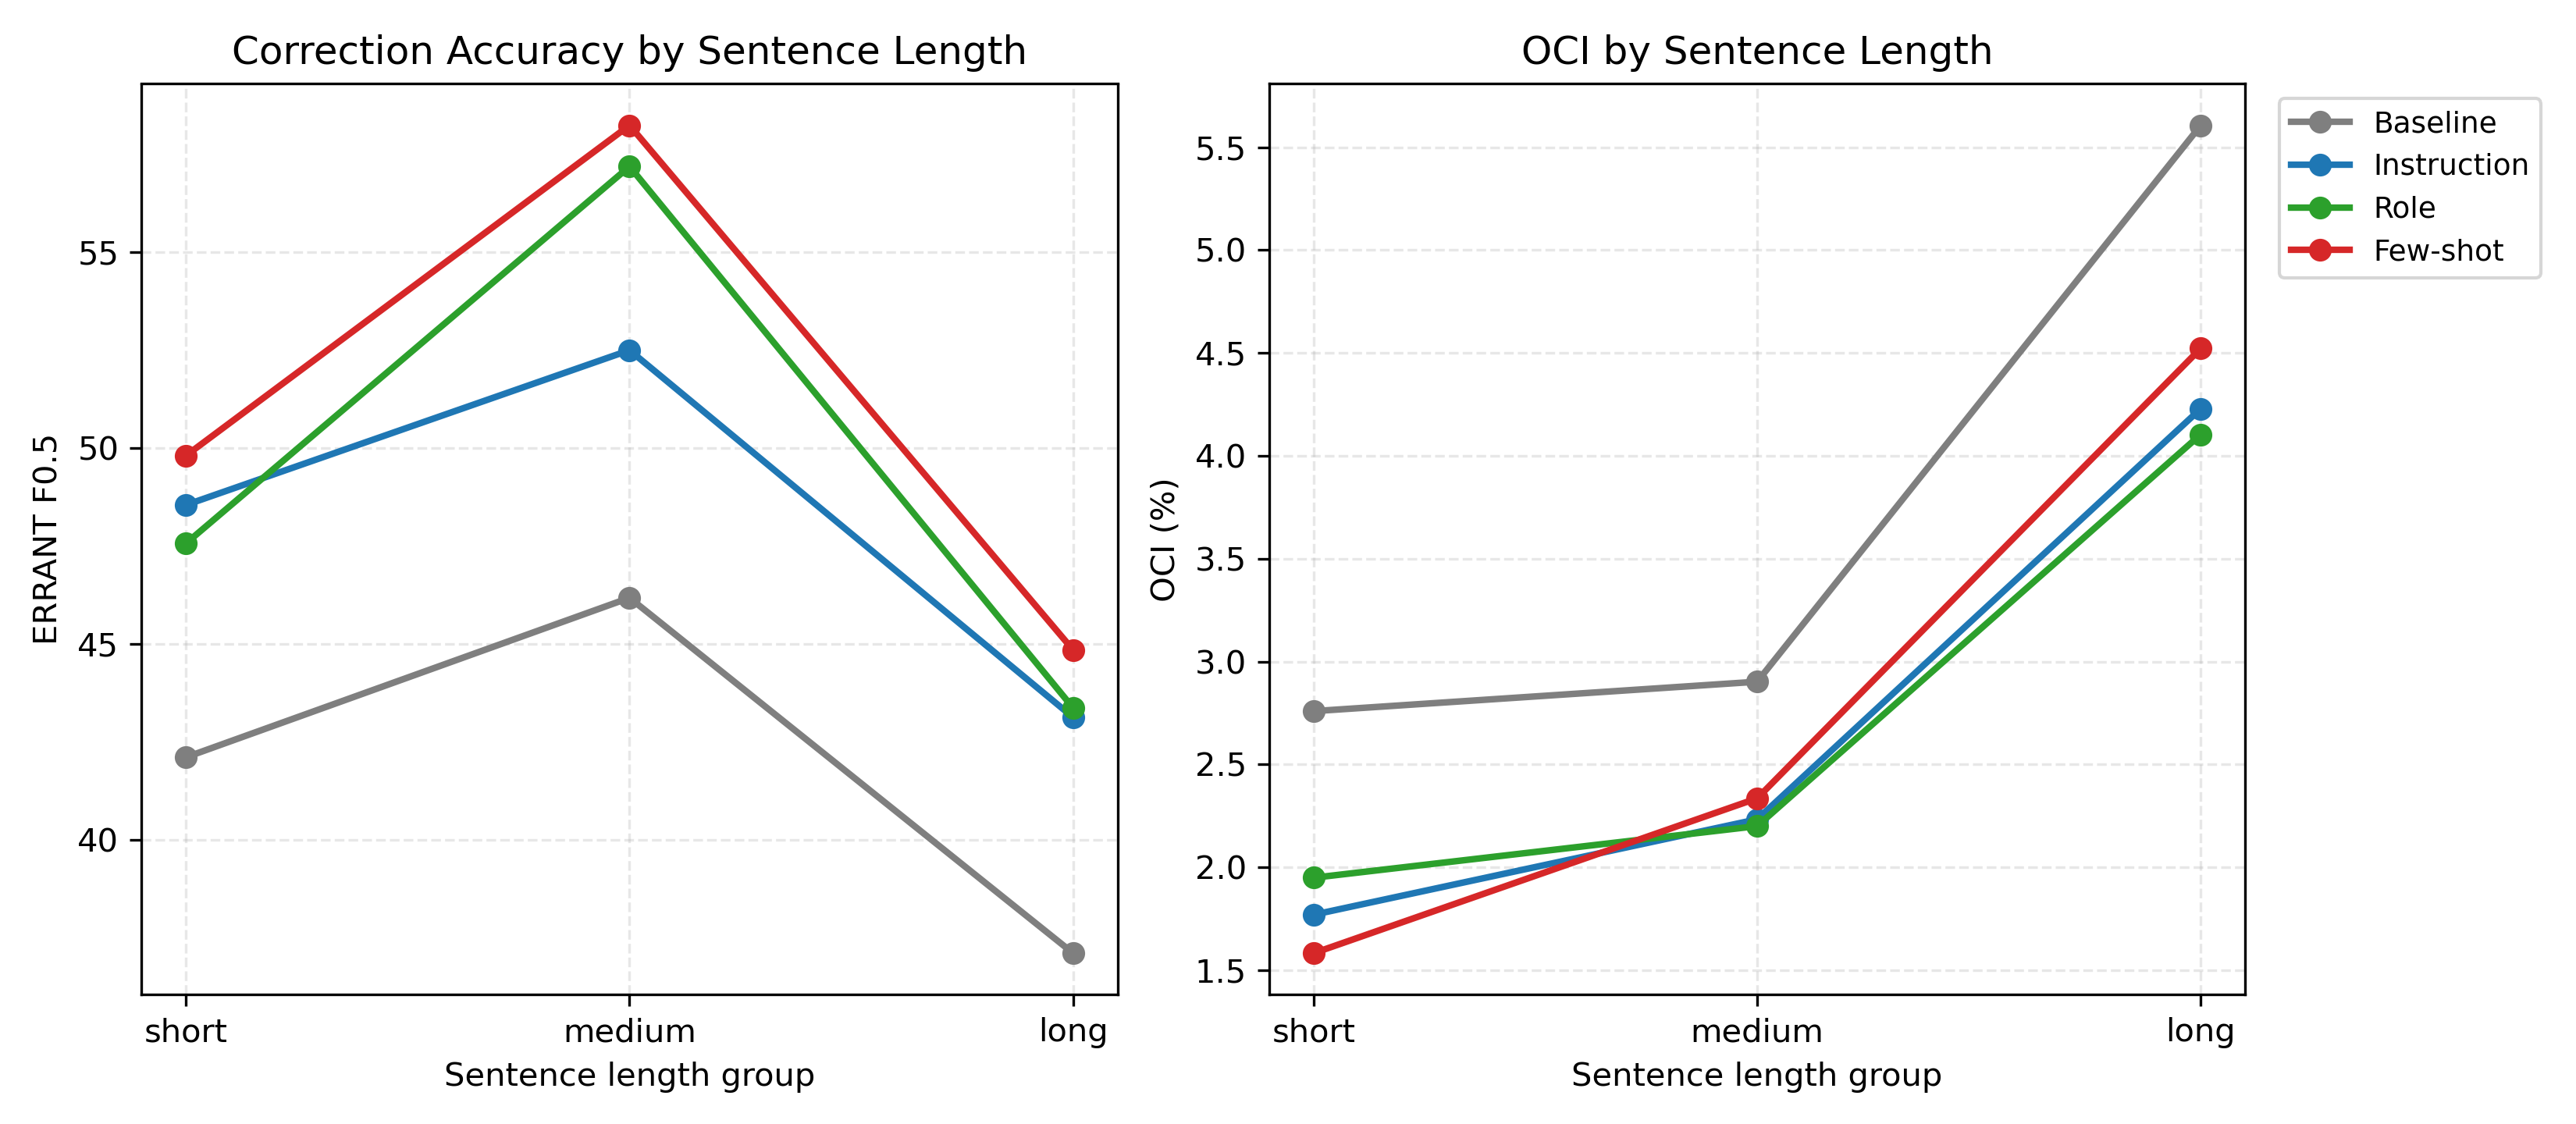
\includegraphics[width=\textwidth]{figures/figure_5_3_sentence_length_all_values.png}
    \caption{Sentence-length effects on correction accuracy and OCI}
    \label{fig:sentence_length_effects}
\end{figure}

Medium-length sentences produced the strongest $F_{0.5}$ scores across all prompt conditions. Few-shot prompting achieved the highest score in this group, 58.24, followed by role-based prompting at 57.19. Long sentences were the most difficult category. The baseline fell to 37.11 $F_{0.5}$ and reached 5.61\% OCI, while every non-baseline prompt remained above 4\% OCI for long sentences.

\subsection{Discussion}

The sentence-length results suggest that over-correction risk is influenced by input complexity as well as prompt design. Medium-length sentences appear to provide enough context for grammatical correction while remaining short enough to avoid major structural rewriting. This helps explain why medium sentences produced the highest $F_{0.5}$ values.

Short sentences produced lower OCI values than long sentences, but they did not always produce the highest correction scores. Short inputs often contain fewer grammatical cues, so the model has less context for deciding whether an edit is required. This can lead either to under-correction or to additional changes with limited apparent utility.

Long sentences remain the main challenge. Their higher OCI values suggest greater over-correction risk when the input is longer. This is consistent with longer sentences creating more opportunities for reorganisation, paraphrasing, or accumulated local edits. The role-based prompt achieved the lowest OCI for long sentences, 4.10\%, suggesting that role-based framing remains the most restrained under complex input conditions.

This result qualifies the main finding. Structured prompting reduces over-correction risk compared with the baseline, but long and complex learner sentences remain difficult. Future systems may therefore benefit from length-adaptive prompts that place stronger emphasis on preserving structure for longer inputs.

\section{Experiment 4: Robustness of the OCI Metric}

\subsection{Purpose}

Experiment 4 tested whether OCI-based conclusions were stable under alternative weighting schemes. This was necessary because OCI is a composite indicator, and its usefulness depends partly on whether prompt rankings remain broadly consistent when component weights are changed.

\subsection{Procedure}

The experiment reused the Experiment 2 metric outputs and recalculated OCI under five weighting schemes: default, edit-heavy, style-heavy, similarity-heavy, and equal weights. The same utility adjustment was applied in each case. For each weighting scheme, prompt conditions were ranked by mean OCI, where rank 1 indicates the lowest over-correction risk.

\subsection{Results}

\begin{table}[htbp]
    \centering
    \caption{OCI prompt rankings under alternative weighting schemes}
    \label{tab:exp4_oci_robustness}
    \renewcommand{\arraystretch}{1.15}
    \begin{adjustbox}{max width=\textwidth}
    \begin{tabular}{lllll}
        \toprule
        \textbf{Weighting scheme} & \textbf{Rank 1} & \textbf{Rank 2} & \textbf{Rank 3} & \textbf{Rank 4} \\
        \midrule
        Default           & Instruction (0.0099) & Role (0.0106) & Few-shot (0.0113) & Baseline (0.0169) \\
        Edit-heavy        & Instruction (0.0107) & Role (0.0112) & Few-shot (0.0115) & Baseline (0.0161) \\
        Style-heavy       & Instruction (0.0091) & Role (0.0098) & Few-shot (0.0107) & Baseline (0.0168) \\
        Similarity-heavy  & Instruction (0.0074) & Role (0.0082) & Few-shot (0.0085) & Baseline (0.0135) \\
        Equal weights     & Instruction (0.0080) & Role (0.0089) & Few-shot (0.0094) & Baseline (0.0151) \\
        \bottomrule
    \end{tabular}
    \end{adjustbox}
\end{table}

\begin{figure}[htbp]
    \centering
    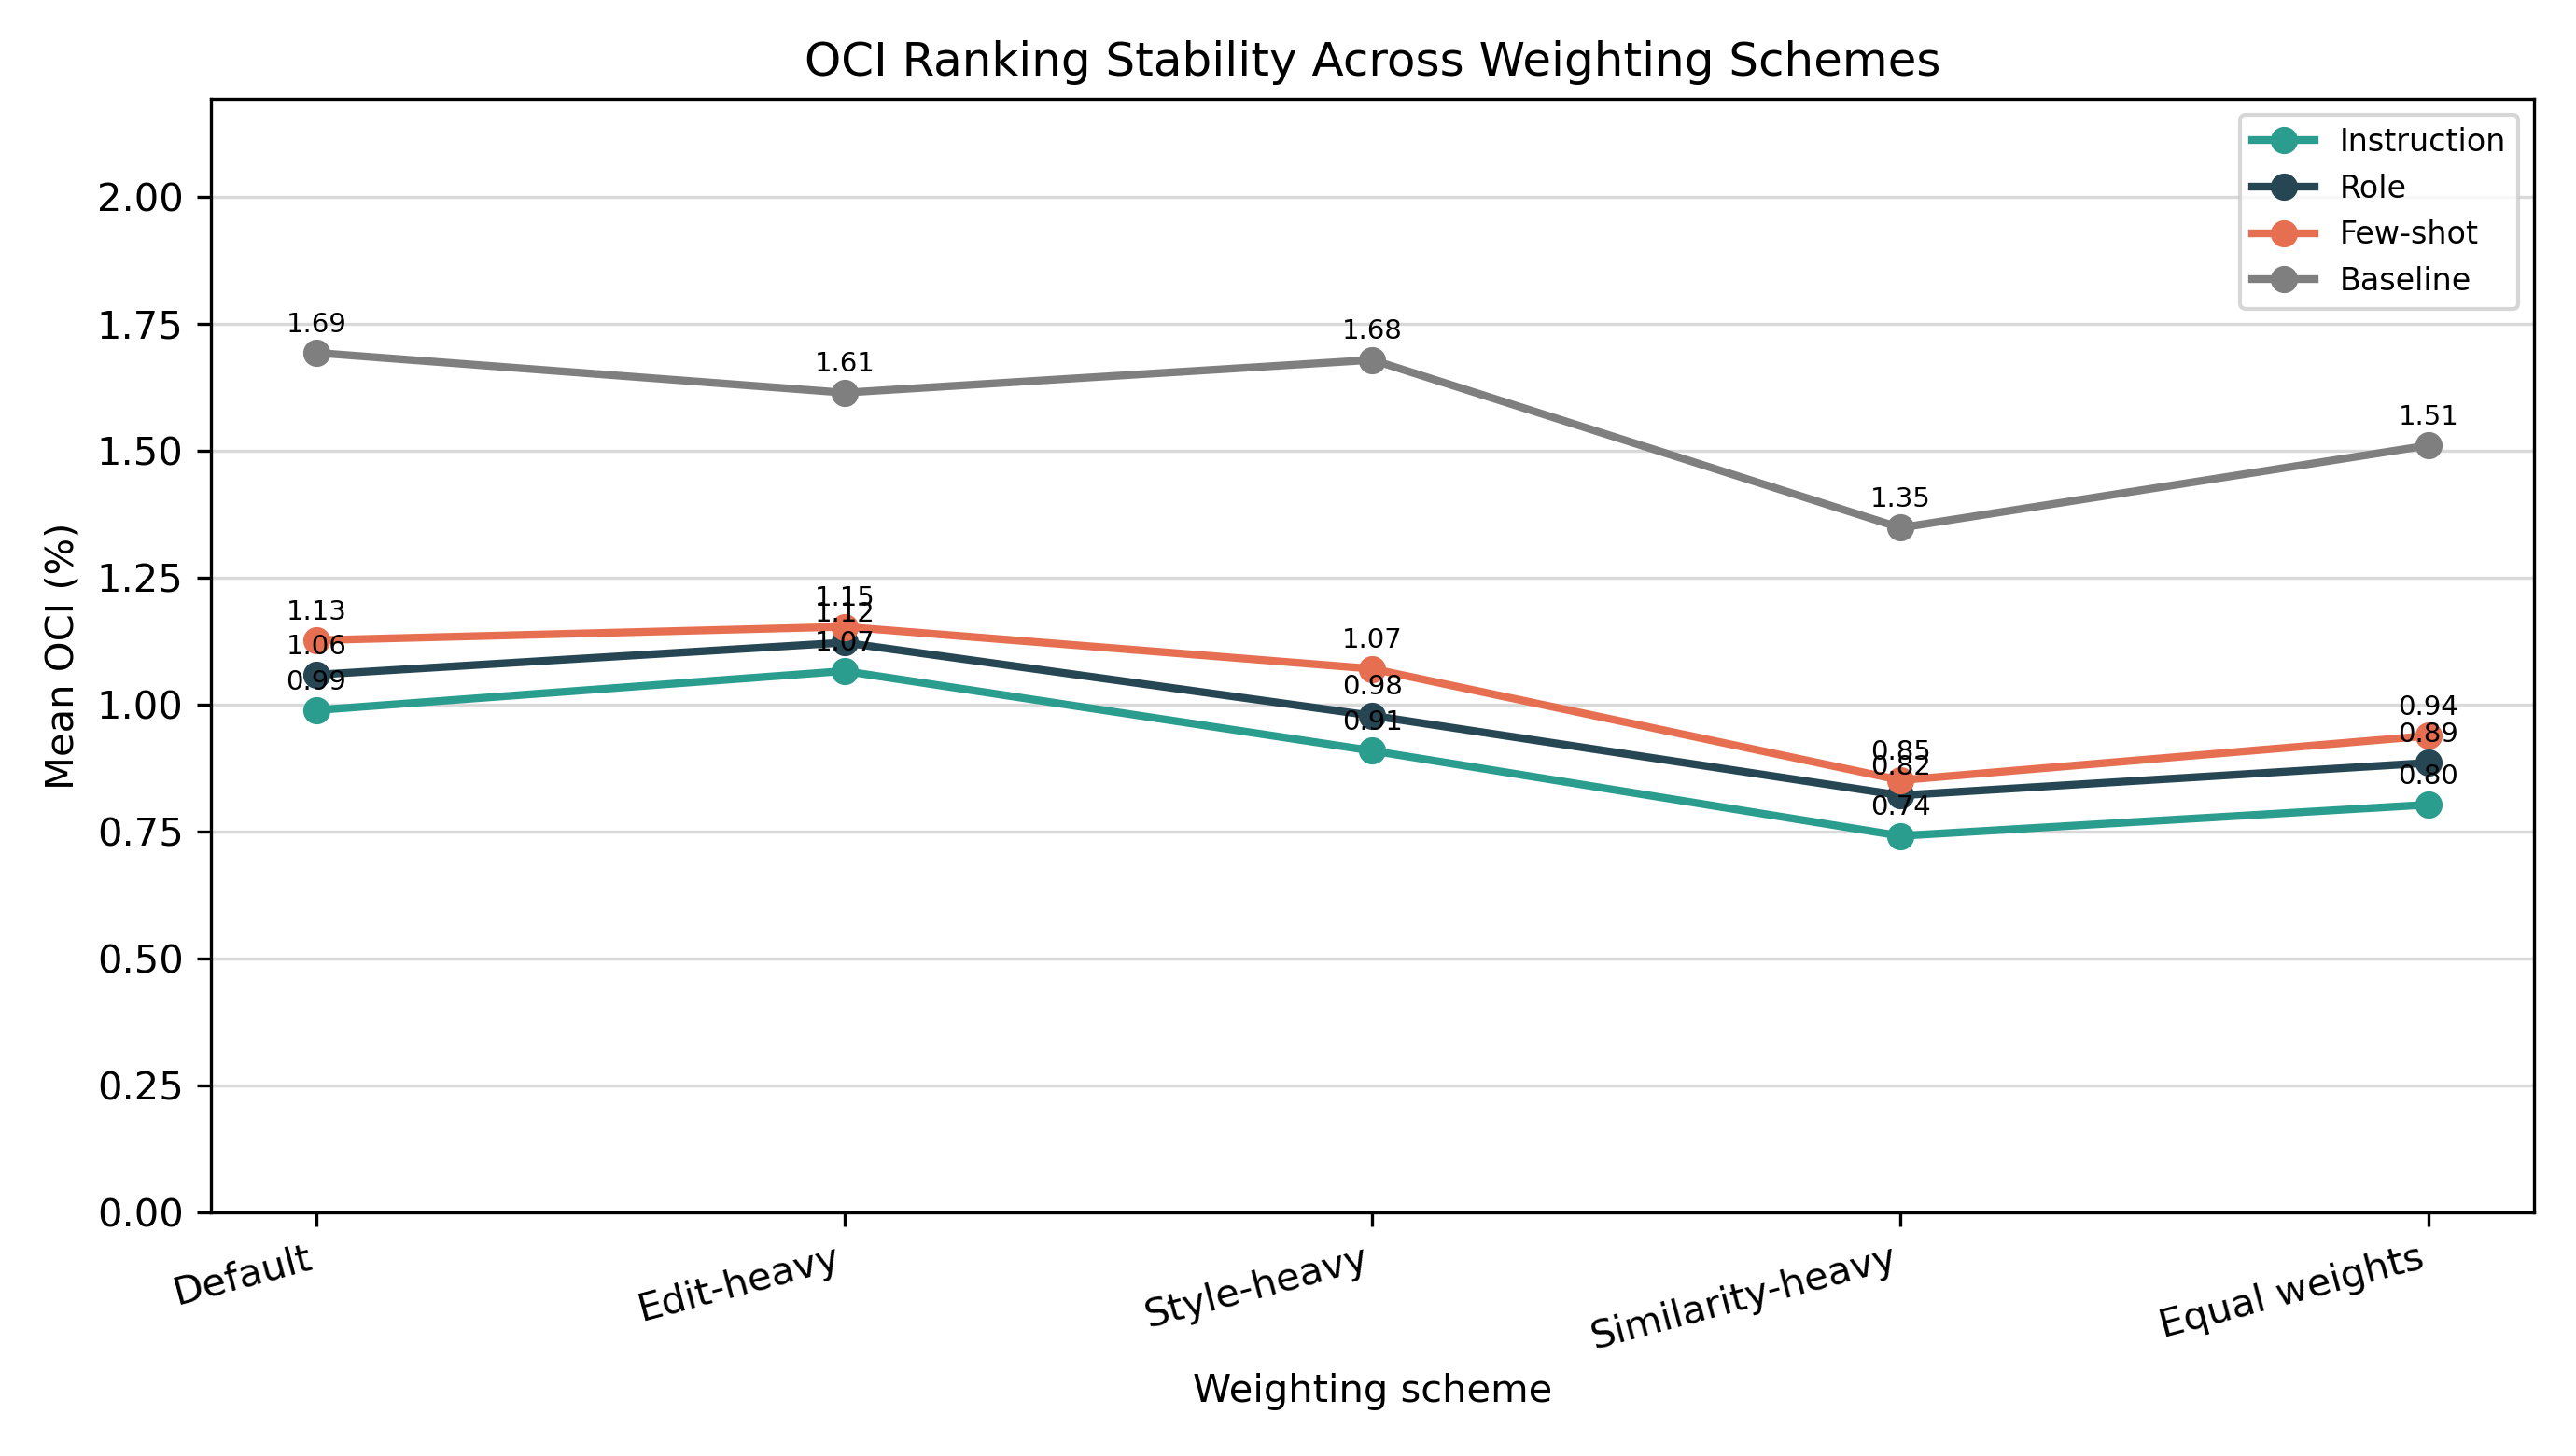
\includegraphics[width=0.86\textwidth]{figures/figure_5_4_oci_robustness.png}
    \caption{OCI ranking stability across weighting schemes}
    \label{fig:oci_robustness}
\end{figure}

The OCI rankings were stable across the alternative weighting schemes. The baseline was ranked last under every weighting scheme, indicating that it produced the highest over-correction risk. Few-shot prompting was consistently ranked third. Instruction ranked first under all five schemes, while role-based prompting ranked second under all five schemes.

\subsection{Discussion}

The robustness analysis strengthens the OCI-based comparison. If prompt rankings had changed substantially under different weights, the metric would be difficult to interpret. Instead, the broad pattern remains stable: the baseline is the least controlled condition, few-shot prompting is more interventionist than instruction-constrained and role-based prompting, and instruction-constrained prompting has the lowest OCI across all weighting schemes.

The relationship between instruction-constrained and role-based prompting should still be interpreted cautiously. Instruction is the most restrained prompt according to OCI, but role-based prompting has stronger correction accuracy. This means the robustness analysis supports instruction-constrained prompting as the lowest-risk option, while Experiment 2 still supports role-based prompting as the strongest balance between correction quality and restraint.

At the same time, this experiment does not make OCI objective in an absolute sense. The weighting schemes test robustness, but the metric still reflects design choices. It is strongest when used for relative comparison between prompts under the same experimental conditions. It is less appropriate as a standalone judgement that a particular individual sentence has definitely been over-corrected.

\section{Experiment 5: Accuracy and Over-Correction Trade-Off}

\subsection{Purpose}

Experiment 5 analyses the relationship between correction accuracy and over-correction risk using the final prompt results from Experiment 2. While Experiment 2 compared prompt strategies directly, this experiment focuses specifically on whether the prompts form a trade-off between ERRANT $F_{0.5}$ and OCI.

The purpose is to determine whether lower over-correction risk necessarily requires sacrificing correction accuracy, or whether some prompt designs improve both dimensions relative to the baseline.

\subsection{Procedure}

The experiment used the $F_{0.5}$ and mean OCI values reported in Experiment 2. Each prompt condition was treated as a point in an accuracy--OCI space, where higher $F_{0.5}$ indicates stronger grammatical correction performance and lower OCI indicates lower over-correction risk.

The analysis compared each structured prompt against the baseline using two quantities: the change in $F_{0.5}$ and the change in OCI. It then examined the structured prompts as a trade-off frontier, identifying whether gains in accuracy were associated with higher OCI.

\subsection{Results}

\begin{table}[htbp]
    \centering
    \caption{Accuracy gain and OCI reduction relative to the baseline}
    \label{tab:exp5_baseline_deltas}
    \renewcommand{\arraystretch}{1.15}
    \begin{adjustbox}{max width=\textwidth}
    \begin{tabular}{lrr}
        \toprule
        \textbf{Condition} & \textbf{$\Delta F_{0.5}$ vs Baseline} & \textbf{$\Delta$ OCI vs Baseline} \\
        \midrule
        Instruction & +6.94 & -0.00704 \\
        Role        & +7.75 & -0.00634 \\
        Few-shot    & +8.92 & -0.00566 \\
        \bottomrule
    \end{tabular}
    \end{adjustbox}
\end{table}

Table~\ref{tab:exp5_baseline_deltas} shows that all structured prompts improve over the baseline on both dimensions. Instruction increases $F_{0.5}$ by 6.94 points while reducing OCI by 0.00704. Role-based prompting increases $F_{0.5}$ by 7.75 points while reducing OCI by 0.00634. Few-shot prompting gives the largest accuracy gain, increasing $F_{0.5}$ by 8.92 points, while still reducing OCI by 0.00566.

This means that the baseline is dominated in the accuracy--OCI space: every structured prompt achieves higher correction performance and lower over-correction risk. Therefore, the results do not support a simple trade-off between accuracy and restraint at the baseline level. Structured prompting improves both compared with the unconstrained baseline.

Among the structured prompts, however, a smaller trade-off appears. Moving from instruction-constrained prompting to role-based prompting increases $F_{0.5}$ by 0.81 points, while OCI increases by 0.00070. Moving from role-based prompting to few-shot prompting increases $F_{0.5}$ by a further 1.17 points, while OCI increases by 0.00068. This indicates that, once prompts are already structured, additional reference-matching accuracy is associated with a small increase in OCI.

\subsection{Discussion}

Experiment 5 adds a trade-off interpretation to the prompt comparison. The main analytical finding is that the baseline is inefficient: it is worse on both dimensions, with lower $F_{0.5}$ and higher OCI than every structured prompt. This shows that over-correction risk is not simply the result of making more useful corrections; the baseline makes more uncontrolled changes without achieving stronger correction performance.

The second finding is that the structured prompts form a small accuracy--OCI frontier. Instruction-constrained prompting represents the lowest-OCI point, few-shot prompting represents the highest-accuracy point, and role-based prompting lies between them. This supports the interpretation that prompt design affects where the model sits in the trade-off space.

This analysis clarifies the conclusion from Experiment 2. Structured prompting can improve both accuracy and over-correction risk relative to a generic baseline. However, among structured prompts, different designs prioritise different behaviours: instruction favours restraint, few-shot prompting favours correction coverage, and role-based prompting provides an intermediate balance.

\section{Experiment 6: Qualitative Analysis}

\subsection{Purpose}

Experiment 6 provides sentence-level examples to support the quantitative results. While $F_{0.5}$ and OCI show measurable differences between prompt conditions, qualitative analysis helps illustrate how potential over-correction appears in actual model outputs.

The aim is not to prove that individual edits are unnecessary, but to show the types of correction behaviour associated with different OCI patterns, including learner-wording preservation, paraphrasing, and style-changing rewrites.

\subsection{Procedure}

The analysis compared baseline outputs with outputs from the role-based prompt, which was the strongest balanced condition in the quantitative experiments. Examples were selected to illustrate three behaviours observed during evaluation: minimal correction that preserves learner-like phrasing, unnecessary paraphrasing, and meaning-preserving but style-changing rewriting.

\subsection{Results}

Table~\ref{tab:qualitative_examples} presents three representative examples comparing baseline and role-based outputs. The examples illustrate minimal correction with learner wording preserved, unnecessary paraphrasing, and meaning-preserving but style-changing rewriting. They are not intended to prove that every baseline edit is unnecessary, but to show the kinds of behaviour that help explain the quantitative OCI patterns.

\begin{table}[htbp]
    \centering
    \caption{Qualitative examples of potential over-correction behaviour}
    \label{tab:qualitative_examples}
    \renewcommand{\arraystretch}{1}
    \begin{adjustbox}{max width=\textwidth}
    \begin{tabularx}{\textwidth}{
        >{\raggedright\arraybackslash}p{0.30\textwidth}
        >{\raggedright\arraybackslash}p{0.33\textwidth}
        >{\raggedright\arraybackslash}p{0.31\textwidth}
    }
        \toprule
        \textbf{Source} & \textbf{Baseline output} & \textbf{Role output} \\
        \midrule
        I am agree with this opinion because it is very important for students to learn English.
        & I agree with this opinion because learning English is essential for students.
        & I agree with this opinion because it is very important for students to learn English. \\
        \addlinespace

        Public transport is not convenient for most of the people because every person wants to reach on time at his place but using public transport it is very difficult to reach on time.
        & Public transport is not convenient for most people because everyone wants to reach their destination on time, but using public transport makes it very difficult to do so.
        & Public transport is not convenient for most of the people because every person wants to reach on time at his place, but using public transport it is very difficult to reach on time. \\
        \addlinespace

        After walking for a lot of days, the survivors were worried, and thinking of how much they would still need to walk to find a city.
        & After walking for many days, the survivors were worried and thinking about how much farther they would need to walk to find a city.
        & After walking for a lot of days, the survivors were worried and thinking of how much they would still need to walk to find a city. \\
        \bottomrule
    \end{tabularx}
    \end{adjustbox}
\end{table}

\subsection{Discussion}

The first example shows that minimal correction can preserve learner-like phrasing. The source sentence contains a clear grammatical error, ``I am agree'', which should be corrected to ``I agree''. The baseline output corrects this error but also rewrites the second clause into a more polished form, changing ``it is very important for students to learn English'' to ``learning English is essential for students''. By contrast, the role-based output corrects the grammatical error while retaining the learner's original wording. This phrasing is understandable but somewhat simple and repetitive, so a human teacher might choose to address it separately as a matter of style rather than grammar.

The second example shows unnecessary paraphrasing. The baseline output changes ``every person'' to ``everyone'' and ``his place'' to ``their destination''. These substitutions improve idiomatic fluency, but they are not required for minimal grammatical correction. The role-based output remains closer to the source sentence, illustrating a more restrained correction style.

The third example shows meaning-preserving but style-changing rewriting. The baseline changes ``thinking of how much they would still need to walk'' to ``thinking about how much farther they would need to walk''. This is not grammatically wrong, but it is more interventionist than necessary for a minimal correction task. The role-based output instead preserves the original phrasing while removing the unnecessary comma.

Together, these examples help explain why the baseline can have high OCI without achieving high $F_{0.5}$. Potential over-correction is associated not only with grammatical edits, but also with lexical substitution, paraphrasing, and fluency-driven rewriting. Such changes may improve surface fluency, but they can reduce feedback transparency by making it harder for the learner to identify the specific grammatical issue being corrected.

The examples also show why automatic metrics need to be interpreted carefully. A fluent rewrite may appear better in isolation, but it can be less appropriate for learner-facing GEC if it removes too much of the learner's wording. Conversely, a minimal correction may preserve awkward phrasing that a human teacher might discuss separately. Overall, the qualitative analysis supports the quantitative finding that the baseline tends to produce broader rewrites, while the role-based prompt more often stays closer to the intended minimal-correction task.

\section{Overall Discussion}

The results indicate that structured prompting can improve the balance between grammatical correction performance and over-correction risk in LLM-based GEC. Across the main prompt comparison, all structured prompts achieved higher $F_{0.5}$ scores and lower OCI values than the baseline, suggesting that prompt design can make correction behaviour more controlled without reducing grammatical performance within this setup.

The prompts also displayed different behavioural profiles. Instruction-constrained prompting produced the lowest OCI and was therefore the most conservative strategy. Few-shot prompting achieved the highest $F_{0.5}$ score, making it the most accuracy-oriented strategy. Within the evaluated setup, role-based prompting provided the strongest overall balance under the chosen evaluation criteria, because it combined the highest precision, strong $F_{0.5}$, the lowest average edit distance, and low OCI.

The sentence-length analysis shows that this improvement is not uniform across all inputs. Long sentences produced higher OCI values across all prompt conditions, suggesting that more complex learner sentences create additional opportunities for restructuring, paraphrasing, or accumulated local edits. This indicates that prompt engineering can reduce over-correction risk, but it does not fully solve the problem for longer or more complex inputs.

The robustness and qualitative analyses support this interpretation. OCI rankings remained stable under alternative weighting schemes, strengthening confidence in the relative comparison between prompts. At the same time, OCI should be interpreted as a comparative indicator rather than a definitive judgement of individual edits. The qualitative examples show why this caution is necessary: fluent outputs may still involve unnecessary paraphrasing, while minimal corrections may preserve learner-like phrasing that is pedagogically useful but not fully polished.

Taken together, the results provide positive but bounded evidence for the research questions. Within the evaluated setup, structured prompts reduced over-correction risk while maintaining or improving grammatical correction performance. Instruction-constrained prompting produced the lowest OCI, few-shot prompting achieved the highest $F_{0.5}$, and role-based prompting provided the strongest overall balance under the chosen evaluation criteria. However, the effect was not uniform across all inputs, and long sentences remained challenging for minimal, learner-facing correction.
